\documentclass[11pt,a4paper]{article}
\usepackage{fontspec}
\setmainfont{DejaVu Sans}[Scale=0.9]
\usepackage{amsmath,amssymb}
\usepackage[left=18mm,right=18mm,top=16mm,bottom=16mm]{geometry}
\usepackage{xcolor,array}
\usepackage{tikz}
\definecolor{grau}{gray}{0.45}
\pagestyle{empty}
\setlength{\parindent}{0pt}
\newcommand{\g}[1]{{\small\color{grau}#1}}
\newcommand{\teil}[2]{\par\filbreak\vspace{12pt}\noindent\makebox[1.6em][l]{\textbf{#1}}\underline{#2}\par\vspace{2pt}}
\newcommand{\sub}[1]{\par\vspace{8pt}\noindent\hspace{1.6em}\underline{#1}\par\vspace{2pt}}
\newcommand{\subsub}[1]{\par\vspace{5pt}\noindent\hspace{3.2em}\underline{#1}\par\vspace{2pt}}
\newcommand{\bem}[1]{\par\noindent\hspace{3.2em}\g{Bem.: #1}\par}
\newcommand{\ansatz}[1]{\noindent\hspace{1.6em}\textit{Ansatz:}\ #1\par\vspace{3pt}}
\newenvironment{weg}{\par\noindent\hspace{3.2em}\renewcommand{\arraystretch}{1.45}\begin{tabular}{@{}l@{\quad}l@{}}}{\end{tabular}\par}
\newcommand{\B}[1]{\boldsymbol{#1}}
\newcommand{\trenn}{\par\vspace{8pt}{\color{grau!50}\hrule}}
\begin{document}
{\large\bfseries 1 Differentialrechnung}\hfill\g{FHR 2026 C · Lösung}\par
\vspace{3pt}\hrule height 1pt\vspace{6pt}
$f(x)=-6x^5+18{,}75x^4+20x^3-90x^2$\par

\teil{a)}{Verhalten im Unendlichen?}
\ansatz{$\lim f(x)=\lim\,(-6x^5)$}
\begin{weg}
$\lim\limits_{x\to-\infty}f(x)=+\infty$, \ $\lim\limits_{x\to+\infty}f(x)=-\infty$ & $\Rightarrow$ Abb.\ 2\,✗, \ 4\,✗\\
\end{weg}
\sub{Verläuft $G_f$ durch $O(0\,|\,0)$?}
\ansatz{$f(0)=0$?}
\begin{weg}
$f(0)=0$ & $\Rightarrow$ ja $\Rightarrow$ Abb.\ 1\,✗\\
 & $\Rightarrow$ \textbf{Abbildung 3 zeigt $G_f$}\\
\end{weg}
\trenn

\teil{b)}{(I) Ist $G_f$ nicht punktsymmetrisch zum Ursprung?}
\ansatz{Geradzahligkeit der Exponenten}
\begin{weg}
Exponenten gerade und ungerade & $\Rightarrow$ ja $\Rightarrow$ (I) \textbf{wahr}\\
\end{weg}
\sub{(II) Liegt jede Nullstelle auf der $y$-Achse?}
\ansatz{$f(a)>0$ und $f(b)<0$ $\Rightarrow$ Nullstelle zwischen $a$ und $b$}
\begin{weg}
$f(-3)\approx1626{,}75>0$; \ $f(-1)=-85{,}25<0$ & $\Rightarrow$ Nullstelle zwischen $-3$ und $-1$\\
 & $\Rightarrow$ nein $\Rightarrow$ (II) \textbf{falsch}\\
\end{weg}
\sub{(III) Mehr Wendestellen als Extremstellen?}
\ansatz{Stellen in Abbildung 3 zählen}
\begin{weg}
3 Wendestellen, 2 Extremstellen & $\Rightarrow$ ja $\Rightarrow$ (III) \textbf{wahr}\\
\end{weg}
\trenn

\teil{c)}{}
\begin{weg}
$\B{f'(x)=-30x^4+75x^3+60x^2-180x}$ & \\
$\B{f''(x)=-120x^3+225x^2+120x-180}$ & \\
$\B{f'''(x)=-360x^2+450x+120}$ & \\
\end{weg}
\trenn

\teil{d)}{Liegt $A(3\,|\,{-200})$ auf $G_f$?}
\ansatz{$y_A\overset{?}{=}f(x_A)$}
\begin{weg}
$f(3)=-209{,}25\neq y_A$ & $\Rightarrow$ \textbf{$A\notin G_f$}\\
\end{weg}
\sub{Liegt $B(-2\,|\,{-28})$ auf $G_f$?}
\ansatz{$y_B\overset{?}{=}f(x_B)$}
\begin{weg}
$f(-2)=-28=y_B$ & $\Rightarrow$ \textbf{$B\in G_f$}\\
\end{weg}
\sub{Tangente in $B$?}
\ansatz{$t(x)=mx+n$ mit $m=f'(x_B)$}
\begin{weg}
$m=f'(-2)=-480$ & $\Rightarrow t(x)=-480x+n$\\
\end{weg}
\subsub{$n$?}
\par\noindent\hspace{3.2em}\textit{Ansatz:} $t(x_B)=f(x_B)$\par\vspace{3pt}
\begin{weg}
$-480\cdot(-2)+n=-28$ & $\Rightarrow n=-988$ $\Rightarrow$ $\B{t(x)=-480x-988}$\\
\end{weg}
\trenn

\teil{e)}{Anstieg null bei $x_1=-1{,}5$, \ $x_2=0$, \ $x_3=2$?}
\ansatz{$f'(x_i)=0$?}
\begin{weg}
$f'(-1{,}5)=f'(0)=f'(2)=0$ & $\Rightarrow$ ja\\
\end{weg}
\sub{Art der Punkte?}
\ansatz{$f''(x_i)>0$ Minimum, \ $f''(x_i)<0$ Maximum, \ $f''(x_i)=0$ und $f'''(x_i)\neq0$ Sattel}
\begin{weg}
$f''(-1{,}5)=551{,}25>0$ & $\Rightarrow$ $x_1$ Minimumstelle\\
$f''(0)=-180<0$ & $\Rightarrow$ $x_2$ Maximumstelle\\
$f''(2)=0$; \ $f'''(2)=-420\neq0$ & $\Rightarrow$ $x_3$ Sattelstelle\\
\end{weg}
\sub{Koordinaten?}
\ansatz{$P(x_i\,|\,f(x_i))$}
\begin{weg}
$f(-1{,}5)\approx-129{,}52$; \ $f(0)=0$; \ $f(2)=-92$ & $\Rightarrow \B{T(-1{,}5\,|\,{-129{,}52})}$, \ $\B{H(0\,|\,0)}$, \ $\B{S(2\,|\,{-92})}$\\
\end{weg}
\sub{Monotonie?}
\ansatz{Vorzeichen von $f'$ zwischen den Stellen \g{(aus $T$, $H$, $S$)}}
\par\vspace{2pt}\noindent\hspace{3.2em}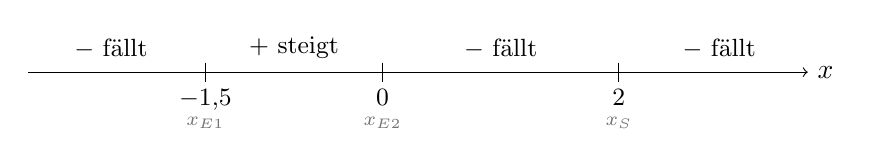
\begin{tikzpicture}[x=1.5cm]
  \draw[->] (-3,0) -- (3.6,0) node[right] {$x$};
  \draw (-1.5,0.12)--(-1.5,-0.12); \node[below,font=\small] at (-1.5,-0.1) {$-1{,}5$}; \node[below,font=\scriptsize,text=grau] at (-1.5,-0.45) {$x_{E1}$};
  \draw (0,0.12)--(0,-0.12); \node[below,font=\small] at (0,-0.1) {$0$}; \node[below,font=\scriptsize,text=grau] at (0,-0.45) {$x_{E2}$};
  \draw (2,0.12)--(2,-0.12); \node[below,font=\small] at (2,-0.1) {$2$}; \node[below,font=\scriptsize,text=grau] at (2,-0.45) {$x_S$};
  \node[above,font=\small] at (-2.3,0.05) {$-$ fällt};
  \node[above,font=\small] at (-0.75,0.05) {$+$ steigt};
  \node[above,font=\small] at (1,0.05) {$-$ fällt};
  \node[above,font=\small] at (2.85,0.05) {$-$ fällt};
\end{tikzpicture}\par\vspace{4pt}
\begin{weg}
 & $\Rightarrow$ \textbf{fällt für $x\le-1{,}5$, steigt für $-1{,}5\le x\le0$, fällt für $x\ge0$}\\
\end{weg}
\trenn

\teil{f)}{Wendestellen im Intervall $-3\le x\le3$?}
\ansatz{$f''(x_W)=0$ und $f'''(x_W)\neq0$}
\begin{weg}
$f''(2)=0$ \ \g{(geraten)} & $\Rightarrow x_{W1}=2$\\
$f''(x):(x-2)=-120x^2-15x+90$ & \\
$x^2+0{,}125x-0{,}75=0$ \ \g{(pq-Formel)} & $\Rightarrow x_{W2}\approx-0{,}93$; \ $x_{W3}\approx0{,}81$\\
$f'''(-0{,}93)\approx-610{,}7$; \ $f'''(0{,}81)\approx248{,}9$; \ $f'''(2)\neq0$ & $\Rightarrow$ alle drei sind Wendestellen\\
\end{weg}
\sub{Koordinaten der Wendepunkte?}
\ansatz{$W(x_W\,|\,f(x_W))$}
\begin{weg}
$\B{W_1(2\,|\,{-92})}$ \ \g{(= $S$)}, \quad $\B{W_2(-0{,}93\,|\,{-75{,}83})}$, \quad $\B{W_3(0{,}81\,|\,{-42{,}11})}$ & \\
\end{weg}
\end{document}
